\documentclass[output=paper]{langscibook}
\ChapterDOI{10.5281/zenodo.5578836}



%This is where you put the authors and their affiliations
\author{Elise Newman\affiliation{MIT}}

%Insert your title here
\title{{\textit{v}P} infinitives in {Wolof}: {On} {\={A}-movement} to {Spec} {\textit{v}P}}  
\abstract{This paper compares two Wolof adjunct clauses, analyzed as relative clauses and purpose clauses respectively, whose comparison is proposed to demonstrate a case of \={A}-movement that terminates at the edge of \textit{v}P. These adjunct clauses are very similar on the surface and have analogous \={A}-dependencies. Despite this similarity, these clauses appear to be different sizes. Evidence from clitic climbing and the distribution of aspect markers suggests that relative clauses are full CPs, while purpose clauses are bare \textit{v}Ps in Wolof. The fact that both clause types can have \={A}-chains with the same profile indicates that \={A}-movement must be able to terminate at Spec \textit{v}P in purpose clauses in the absence of a higher probe. This requires a theory in which \={A}-movement to Spec \textit{v}P is independent of further movement to Spec CP. Constituency tests further support an analysis of purpose clauses in Wolof as parasitic gap constructions.}

\begin{document}
\SetupAffiliations{mark style=none}
\maketitle

\section{Introduction} \label{sec:newman:intro}



In this paper, I discuss the properties of two types of Wolof adjunct clauses that have a very similar surface form. One of these clauses has the canonical form of a relative clause in Wolof, while the other will be argued to be smaller and structurally higher. Wolof is an Atlantic language spoken primarily in Senegal and The Gambia. It is characterized by SVO word order and noun classes. The data in this paper are from original fieldwork conducted in Boston with three speakers of Wolof, who are originally from Kaolack and Dakar.

The adjunct clauses I will focus on are presented in \REF{ex:newman:bu}, which were both elicited in a context that an English speaker would describe with an infinitival relative clause. These examples differ on the surface only in the presence or absence of a relativizing head \emph{bu}. Note that all examples are written in Wolof, rather than IPA.

\begin{exe}
	\ex \label{ex:newman:bu} \begin{xlist}
		\ex 
		\gll Kadeer jox na ma j\"en [\textbf{b-u} ma jox Roxaya] \\
		K give \textsc{3sg.pfv} me fish \textsc{cl-rel} \textsc{1sg} give R \\
		\trans `Kadeer gave me a fish to give to Roxaya.'
		\ex 
		\gll Kadeer jox na ma j\"en [ma jox Roxaya] \\
		K give \textsc{3sg.pfv} me fish \textsc{1sg} give R \\
		\trans `Kadeer gave me a fish to give to Roxaya.'
	\end{xlist}
\end{exe}

Despite the surface similarity of (\ref{ex:newman:bu}a,b), the presence or absence of \emph{bu} has syntactic consequences. Adjuncts with \emph{bu} require clitic arguments to move across the verb. Their \emph{bu}-less counterparts, however, leave clitic arguments in situ. This is demonstrated in \REF{ex:newman:clitic}, which contain a clitic (in bold), whose position depends on the presence of \emph{bu}.

\begin{exe}
	\ex \label{ex:newman:clitic} \begin{xlist}
		\ex[]{ 
		\gll Kadeer jox na ma j\"en [\textbf{b-u} ma \textbf{ko} jox] \\
		K give \textsc{3sg.pfv} me fish \textsc{cl-rel} \textsc{1sg} her give \\
		\trans `Kadeer gave me a fish to give to her.'}
		\ex[*]{ 
		\gll Kadeer jox na ma j\"en [ma \textbf{ko} jox] \\
		K give \textsc{3sg.pfv} me fish \textsc{1sg} her give \\
		\trans `Kadeer gave me a fish to give to her.'}
		\ex[]{
		\gll Kadeer jox na ma j\"en [ma jox \textbf{ko}] \\
		K give \textsc{3sg.pfv} me fish \textsc{1sg} give her \\
		\trans `Kadeer gave me a fish to give to her.'}
	\end{xlist}
\end{exe}

Additionally, the presence of \emph{bu} appears to license the presence of aspectual heads in the clause. By contrast, overt aspect is ruled out in \emph{bu}-less infinitives.

\begin{exe}
	\ex 
	\gll Roxaya jox na Kadeer j\"en [*(b-u) mu-y togg] \\
	R give \textsc{3sg.pfv} K fish \textsc{cl-rel} \textsc{3sg-ipfv} cook \\
	\trans `Roxaya gave Kadeer a fish to cook (habitually).'
\end{exe}

\begin{table}
\begin{tabular}{ l  c  c }
\lsptoprule
Clause type & \emph{bu}-full & \emph{bu}-less \\ 
\midrule
Supports aspect & \langscicheckmark & * \\ 
Clitics climb & \langscicheckmark & * \\ 
\lspbottomrule
\end{tabular}
\caption{Summary of the properties of these two clauses}
\end{table}

Based on these data, I will argue that the presence or absence of \emph{bu} is not governed by true optionality, but rather correlates with a difference in clause size. Following \citet{martinovic:2015}, I will assume that clitics in Wolof climb to the right of the highest functional head in their phase, which she argues is the C/T complex in finite clauses, but \textit{v} in non-finite clauses. The fact that \emph{bu}-less clauses lack clitic climbing therefore suggests that these clauses are bare \textit{v}Ps. The presence of \emph{bu}, however, extends the clause to a full CP and thus causes clitics to climb. This proposal also accounts for the variable behavior of these clauses with respect to hosting aspect. Full CPs are able to host aspect, but bare \textit{v}Ps are not. 

I will ultimately argue that examples like (\ref{ex:newman:bu}a) are regular relative clauses while examples like (\ref{ex:newman:bu}b) are not, but are rather a sort of purpose clause. I assume an operator movement approach to relative clauses, taking \REF{ex:newman:baseline} to be a baseline derivation for sentences like (\ref{ex:newman:bu}a). This derivation involves successive cyclic operator movement from the complement of V through Spec \textit{v}P and finally landing in Spec CP. 

\begin{exe}
	\ex \label{ex:newman:baseline} % 
		\tikzstyle{every picture}+=[remember picture, inner sep=0pt, baseline, anchor=base]%
		Proposed derivation for adjunct clauses with \emph{bu}\\
		{} Kadeer jox na ma j\"en$_i$ $[_{CP}$ \tikz\node(op){\emph{Op$_i$}}; $[$ \textbf{bu} ma ... $[_{vP}$ \tikz\node(node2){$t$}; $[$ jox Roxaya \tikz\node(node1){<gap>}; $] ] $\\
\begin{tikzpicture}[overlay]
\draw[-latex] (node1.south) -- ++(south:1.5ex) -| (node2.south);
\draw[-latex] (node2.south) -- ++(south:1.5ex) -| (op.south);
\end{tikzpicture}
\end{exe}

I will propose that examples like (\ref{ex:newman:bu}b) likewise involve \={A}-movement but only to Spec \textit{v}P, based on the observation that both clauses with and without \emph{bu} contain gaps with \={A}-properties. Evidence for this can be seen in two parts. The variety of Wolof discussed here has two strategies for long distance \={A}-movement, one with resumption and one without. We first observe that attempting to embed the gaps in either of the examples in \REF{ex:newman:bu} requires resumption. However, these resumptive pronouns can be shown to be island sensitive, thus suggesting that they are nonetheless derived by movement. These facts combined argue for an analysis in which both (\ref{ex:newman:bu}a,b) have gaps derived by \={A}-movement, despite the fact that the clauses in each example are different sizes.

\begin{exe}
	\ex % 
		\tikzstyle{every picture}+=[remember picture, inner sep=0pt, baseline, anchor=base]%
		Proposed derivation for \emph{bu}-less clauses\\
		{} Kadeer jox na ma j\"en$_i$ $[_{\textit{vP}}$ \tikz\node(op){\emph{Op$_i$}}; \tikz\node(node2){ma}; $[$ jox Roxaya \tikz\node(node1){<gap>}; $] ] $\\
		\begin{tikzpicture}[overlay]
\draw[-latex] (node1.south) -- ++(south:1.5ex) -| (op.south);
\end{tikzpicture}
\end{exe}

This finding has a theoretical consequence regarding the nature of \={A}-move\-ment. If the above reasoning is correct, the infinitival clause in (\ref{ex:newman:bu}b) should be analyzed as a \textit{v}P-sized adjunct clause containing a gap derived by \={A}-movement. However, the only possible clause-internal \={A}-position is Spec \textit{v}P. This not only supports theoretical claims and empirical findings that \={A}-movement is successive cyclic through \textit{v}P, but also provides evidence that \={A}-movement can \emph{terminate} at the edge of \textit{v}P, which has consequences for theories of what drives successive cyclic movement to begin with.



The outline of this paper is as follows: \sectref{sec:newman:cc} presents background on relative clauses and clitic climbing patterns in Wolof, showing why clitic climbing is a good diagnostic for clause size;  \sectref{sec:newman:abar} diagnoses \={A}-movement in both the \emph{bu} and \emph{bu}-less clauses; and finally, \sectref{sec:newman:vpinfs} presents constituency tests and suggests a possible analysis for the \emph{bu}-less clauses as a parasitic gap construction.


\section{Relative clauses and clitic climbing} \label{sec:newman:cc}



Relative clauses in Wolof typically contain a relativizing head that matches the noun class of the head nominal. This can be seen in \REF{ex:newman:relt}, where the class marker on the relativizer agrees with the class marker on the indefinite article.

\begin{exe}
    \ex \label{ex:newman:relt} \citep[104--106]{torrence:2013}\begin{xlist}
        \ex 
        \gll (u-\textbf{j}) y\`ambaa \textbf{j}-u \~nu t\'ox\\
        \textsc{ndef-cl} marijuana \textsc{cl-rel} \textsc{3pl} smoke\\
        \glt `some marijuana that they smoked'
        \ex
        \gll (u-\textbf{m}) p\'o\'on \textbf{m}-u \~nu t\'ox\\
        \textsc{ndef-cl} tobacco \textsc{cl-rel} \textsc{3pl} smoke\\
        \glt `some tobacco that they smoked'
    \end{xlist}
\end{exe}

I will assume with \citet{torrence:2013}, that these relativizing heads are complementizers, which suggests that relative clauses are full CPs in Wolof. A puzzling feature of this result is that there is no overt tense morphology inside Wolof relative clauses. Despite this, they seem to carry a default past interpretation.

If a speaker wants to indicate a non-past interpretation explicitly, adding an imperfective marker gives the relative clause an infinitival interpretation, despite the lack of an overt non-finite element. However, in my elicitation sessions, speakers often accepted (\ref{ex:newman:tense}a) in contexts like (\ref{ex:newman:tense}b), suggesting that they may be truly tense-less. 

\begin{exe}
    \ex \label{ex:newman:tense} \begin{xlist}
        \ex 
        \gll Kadeer jox na ma j\"en b-u ma jox Roxaya\\
        K give \textsc{3sg.pfv} me fish \textsc{cl-rel} \textsc{1sg} give R\\
        \glt Default: `Kadeer gave me a fish that I gave to Roxaya.'
        \ex 
        \gll Kadeer jox na ma j\"en b-u ma-\textbf{y} jox Roxaya\\
        K give \textsc{3sg.pfv} me fish \textsc{cl-rel} \textsc{1sg-ipfv} give R\\
        \glt Comment: `I haven't given her the fish yet.'
    \end{xlist}
\end{exe}

The tense properties of Wolof relative clauses deserve much further scrutiny. In this paper, however, I want to focus on the structural relevance of the relativizing head, rather than the content of the functional projections in its scope. 

Torrence argues that the relativizing head is obligatory in \REF{ex:newman:relt}, unlike English relativizers, a conclusion which is apparently contradicted in \REF{ex:newman:bu}. I argue, however, that this contradiction is only apparent, and that the two clauses are structurally distinct given evidence from clitic climbing.

\begin{exe}
	\exr{ex:newman:bu} \begin{xlist}
		\ex 
		\gll Kadeer jox na ma j\"en [\textbf{b-u} ma jox Roxaya] \\
		K give \textsc{3sg.pfv} me fish \textsc{cl-rel} \textsc{1sg} give R \\
		\trans `Kadeer gave me a fish to give to Roxaya.'
		\ex 
		\gll Kadeer jox na ma j\"en [ma jox Roxaya] \\
		K give \textsc{3sg.pfv} me fish \textsc{1sg} give R \\
		\trans `Kadeer gave me a fish to give to Roxaya.'
	\end{xlist}
\end{exe}

Wolof has what others have called both ``weak'' and ``strong'' pronouns. I'll henceforth refer to the weak pronouns as \emph{clitics} \citep{dunigan:1994,torrence:2005,russel:2006,martinovic:2015}. We will primarily be concerned with object clitics.


\begin{table}[H]
\begin{center}
\begin{tabular}{ c  c  c }
\lsptoprule
Person & Singular & Plural\\
\midrule
1st & ma & nu \\ 
2nd & la & leen \\ 
3rd & ko & leen \\ 
\lspbottomrule
\end{tabular}
\caption{Full paradigm of object clitics in Wolof}
\end{center}
\end{table}

Wolof weak object pronouns behave like clitics in that they have positional requirements that differ from their corresponding full nominals. Sometimes they appear ``in situ'' to the right of the verb, but can also occur preverbally following certain tense, aspect or information structural particles. Wolof expresses subject agreement on such TMA and information structural particles, leading to some debate regarding the correct treatment of them. Our consultants referred to these particles as \emph{subjects} so I will adopt this terminology in part and refer to them as \emph{subject particles} (henceforth SP), in order to remain agnostic about their theoretical description. In \REF{ex:newman:situ} and \REF{ex:newman:climb}, we see that object clitics always surface to the right of SPs, irrespective of whether they precede or follow the verb. By contrast, full DP objects always surface to the right of the verb, regardless of where the SP is.\footnote{I chose to demonstrate the clitic climbing pattern in embedded clauses because the contexts were easier to isolate for the speakers this way. However, the pattern is general to matrix clauses as well (i.e. \emph{Roxaya daf ko lekk} is also good = ``R ate it'', but not \emph{*Roxaya dafa lekk ko}.).}


\begin{exe}
\multicolsep=.25\baselineskip
\ex \label{ex:newman:situ}Post-verbal SP \textsc{na} (perfective, neutral focus): DPs and clitics next to \textsc{na}
	\begin{xlist}
		\ex
		\gll Roxaya lekk \emph{na} \textbf{mango} \textbf{bi} \\ 
		R eat \textsc{3sg.pfv} mango \textsc{def} \\ 
		\trans `Roxaya ate the mango.'
		\ex 
		\gll Roxaya lekk \emph{na} \textbf{ko} \\ 
		R eat \textsc{3sg.pfv} it \\
		\trans `Roxaya ate it.'
	\end{xlist}
	
\ex \label{ex:newman:climb}
	Pre-verbal SPs \textsc{moo, dafa, dina} (subject focus, verb focus, future): Only clitics next to SP\\
	\gll Roxaya wax na ma ne...\\
	R say \textsc{3sg.pfv} me that...\\
	\trans `Roxaya told me that...'
	\begin{multicols}{2}
	\begin{xlist}
		\ex 
		\gll \emph{moo} lekk \textbf{mango} \textbf{bi} \\ 
		 3\textsc{sg.sbj-foc} eat mango \textsc{def} \\
		\trans `SHE ate the mango.'
		\ex 
		\gll \emph{dafa} lekk \textbf{mango} \textbf{bi}\\
		3\textsc{sg.v-foc} eat mango \textsc{def} \\
		\trans `she ATE the mango.'
		\ex 
		\gll \emph{dina} lekk \textbf{mango} \textbf{bi}\\
		3\textsc{sg.fut} eat mango \textsc{def}\\
		\trans `she will eat the mango.'
		\ex
		\gll  \emph{moo} \textbf{ko} lekk \\ 
		 3\textsc{sg.sbj-foc} it eat \\
		\trans `SHE ate it.'
		\ex 
		\gll \emph{daf} \textbf{ko} lekk\\
		3\textsc{sg.v-foc} it eat \\
		\trans `she ATE it.'

		\ex 
		\gll \emph{dina} \textbf{ko} lekk \\
		3\textsc{sg.fut} it eat\\
		\trans `she will eat it.'

	\end{xlist}
	\end{multicols}
\end{exe}

\citet{martinovic:2015} shows that the variable order of SPs and the verb can be understood if the preverbal SPs are morphologically more complex than \textsc{na}. In her view, the preverbal SPs have the status of auxiliaries, which block movement of the verb to C/T. By contrast, \textsc{na} does not trigger insertion of an auxiliary and allows the verb to move high.

On this view, Martinovi\'c accounts for the distribution of clitics by proposing that clitics must always adjoin to the sister of the highest phase head, which for her is the C/T complex. This proposal straightforwardly extends to the examples in \REF{ex:newman:climb}. Assuming that preverbal SPs are high (either because they were generated high or moved high), clitics should have to adjoin to them and are therefore correctly predicted to appear to the left of a verb that remains in \textit{v}P. 

\begin{exe}
	\ex % 
		\tikzstyle{every picture}+=[remember picture, inner sep=0pt, baseline, anchor=base]%
		{} $[_{\textit{C/TP}}$ \emph{subject} $[_{\textit{C/T}}$ \tikz\node(node3){\emph{moo-}}; \tikz\node(node4){\textit{ko}}; $[$ ... $[_{\textit{vP}}$ \tikz\node(node2){$t_{\textit{subj}}$}; V \tikz\node(node1){$t_{\textit{ko}}$}; $] ] ]$ \hfill \emph{Clitics move to C/T, i.e. SP}\\
		\begin{tikzpicture}[overlay]
\draw[-latex,overlay] (node1.south) -- ++(south:1.5ex) -| (node4.south);
\end{tikzpicture}
\end{exe}

Provided that the verb is higher in \REF{ex:newman:situ} than it is in \REF{ex:newman:climb}, clitics are likewise expected to move to the right of the SP \textsc{na}, though this movement does not have apparent word order effects. Looking at ditransitives confirms that the clitic does indeed move to \textsc{na}. While ditransitives typically display free word order between the two internal argument DPs, clitic arguments of ditransitives (regardless of thematic role) are required to be adjacent to the verb\footnote{Clitics also have a fixed hierarchy that determines their ordering in a cluster: 1st person \textgreater{} 2nd person \textgreater{} 3rd person plural \textgreater{} 3rd person singular \textgreater{} locative \emph{fa/fi}, which is potentially relevant to an analysis of clitic climbing but will not bear on the proposal here.}. This suggests that clitics move to the right of \textsc{na}.



\begin{exe}
\ex \begin{xlist}
		\ex[]{
		\gll jox \emph{naa} $[$xale yi teere bi$]$ \\
		give \textsc{1sg.pfv} child \textsc{def.pl} book \textsc{def} \\}
		\ex[]{
		\gll jox \emph{naa} $[$teere bi xale yi$]$ \\ 
		give \textsc{1sg.pfv} book \textsc{def} child \textsc{def.pl} \\
		\trans `I gave the children the book.'}
		\ex[*]{
		\gll jox \emph{naa} $[$xale yi \textbf{ko}$]$ \\
		give \textsc{1sg.pfv} child \textsc{def.pl} it \\}
		\ex[]{
		\gll jox \emph{naa} $[$\textbf{ko} xale yi$]$ \\
		give \textsc{1sg.pfv} it child \textsc{def.pl} \\
		\trans `I gave it to the children.'}
	\end{xlist}
\ex Proposed structure of \textsc{na}-clauses\\
		\tikzstyle{every picture}+=[remember picture, inner sep=0pt, baseline, anchor=base]%
		{} $[_{\textit{C/TP}}$ \emph{subject} $[_{\textit{C/T}}$ \tikz\node(node3){V-\textsc{na}-}; \tikz\node(node4){$\textit{ko}$}; $[$ ... $[_{vP}$ $t_{\textit{subj}}$ \tikz\node(node2){$t_V$}; \tikz\node(node1){$t_{\textit{ko}}$}; $] ] ]$ \hfill \emph{Clitics and V move to \textsc{na}}\\
		\begin{tikzpicture}[overlay]
\draw[-latex] (node1.south) -- ++(south:1.5ex) -| (node4.south);
\draw[-latex] (node2.south) -- ++(south:2ex) -| (node3.south);
\end{tikzpicture}
\end{exe}


Additional support for Martinovi\'c's proposal that clitics move to the right of the highest phase head comes from non-finite clauses. In non-finite clauses, clitics show sensitivity to the presence of functional structure above \textit{v}P. We saw that in finite clauses, clitics always move next to the SP in the clause. In non-finite clauses however, clitics typically stay in situ, separated by the verb from the infinitival SP \textsc{mu}.

\begin{exe}
	\ex \label{neg} \begin{xlist}
		\ex []{
		\gll Roxaya wax na Kadeer [\emph{mu} togg-al \textbf{ko} j\"en] \\
		R say \textsc{3sg.pfv} K \textsc{3sg} cook-\textsc{ben} her fish \\}
		\ex[*]{
		\gll Roxaya wax na Kadeer [\emph{mu} \textbf{ko} togg-al j\"en] \\
		R say \textsc{3sg.pfv} K \textsc{3sg} her cook-\textsc{ben} fish \\
		\trans `Roxaya told Kadeer to cook her fish.'}
	\end{xlist}
\end{exe}	

\textsc{mu} is used in a variety of biclausal constructions such as control predicates, relative clauses, and subjunctive clauses. It behaves more like a subject pronoun than the other SPs in that it is in complementary distribution with an overt external argument within the clause, instead controlled by an antecedent in the superordinate clause. \textsc{mu} is also in complementary distribution with other SPs that carry tense information, which is what we expect for a tense-less clause. 

\begin{exe}
	\ex 
	\gll Roxaya b\'ayyi na Kadeer [\emph{mu} j\"{e}nd \textbf{ko}]\\
	R let \textsc{3sg.pfv} K \textsc{3sg} buy it\\
	\trans `Roxaya let Kadeer buy it.'
	\ex
	\gll B\"{e}gg naa [mu taw]\\
	want \textsc{1sg.pfv} \textsc{3sg} rain\\
	\trans `I want it to rain.'
\end{exe}

Clitics may move next to \textsc{mu} in the presence of additional projections, however. If one adds imperfective aspect or negation to the infinitival clause, the clitic suddenly climbs to the right of \textsc{mu}, thus patterning with finite clauses. 

\begin{exe}
	\ex \begin{xlist}
		\ex
		\gll Roxaya wax na Kadeer [\emph{mu} \textbf{ko}-y togg-al j\"en] \\
		R say \textsc{3sg.pfv} K \textsc{3sg} her-\textsc{ipfv} cook-\textsc{ben} fish \\
		\trans `Roxaya told Kadeer to cook her fish (habitually).'
		\ex
		\gll Roxaya wax na Kadeer [b-u(l) \emph{mu} \textbf{ko} togg-al j\"en] \\
		R say \textsc{3sg.pfv} K \textsc{cl-C$_{\textit{neg}}$} \textsc{3sg} her cook-\textsc{ben} fish \\
		\trans `Roxaya told Kadeer not to cook her fish.'
	\end{xlist}
\end{exe}

Martinovi\'c explains this pattern by concluding that \textsc{mu}-clauses are typically bare \textit{v}Ps (she calls these ``minimal clauses''). In a bare \textit{v}P clause, \textit{v} is the highest head in the phase, attracting both the verb and the object clitic, and resulting in VO order. The \textsc{mu} SP, which acts like a subject pronoun, is argued to be projected in Spec \textit{v}P as a normal subject, and is thus separated from the object clitic by the verb. 

Adding additional projections such as aspect or negation extends the clause (and perhaps the phase boundary) so that the object clitic and clitic-like \textsc{mu} must climb past the verb, which remains in \textit{v}. 

\begin{exe}
	\ex % 
		\tikzstyle{every picture}+=[remember picture, inner sep=0pt, baseline, anchor=base]%
		{} $[$ \tikz\node(node3){\textit{mu}}; \tikz\node(node4){\textit{ko}}; $[_{\textit{XP}}$ ... $[_{\textit{vP}}$ \tikz\node(node2){$t_{\textit{mu}}$}; V \tikz\node(node1){$t_{\textit{ko}}$}; $] ] ]$ \hfill \emph{Clitics only climb in clauses bigger than \textit{v}P}\\
		\begin{tikzpicture}[overlay]
\draw[-latex] (node1.south) -- ++(south:1.5ex) -| (node4.south);
\draw[-latex] (node2.south) -- ++(south:2ex) -| (node3.south);
\end{tikzpicture}
\end{exe}

In summary, Martinovi\'c's approach shows that clitic climbing can be a good diagnostic for clause size in Wolof, given its sensitivity to the presence of negation/aspectual structure above \textit{v}P. I therefore assume with Martinovi\'c that finite clauses in Wolof are full CPs, so clitics always move to the right of the C/T complex (which contains the SP). Non-finite clauses are bare \textit{v}Ps, which typically means that clitics only move a short distance to the right of the verb, thus separated from the SP \textsc{mu}, which is proposed to be in Spec \textit{v}P. However, we see both move further in the presence of additional functional structure above the verb, such as negation or aspect. 

Recalling the initial puzzle, if we construct a relative clause, we see that the presence or absence of the relativizing complementizer affects whether an object clitic in that clause climbs. Following the above assumptions about clitic climbing, this suggests that the \emph{bu}-less clauses lack any structure above \textit{v}P, as evidenced by the fact that clitic climbing is blocked.

\begin{exe}
	\exr{ex:newman:clitic} \begin{xlist}
		\ex []{
		\gll Kadeer jox na ma j\"en [\textbf{b-u} \emph{ma} \textbf{ko} jox] \\
		K give \textsc{3sg.pfv} me fish \textsc{cl-rel} \textsc{1sg} her give \\
		\trans `Kadeer gave me a fish to give to her.'}
		\ex [*]{
		\gll Kadeer jox na ma j\"en [\emph{ma} \textbf{ko} jox] \\
		K give \textsc{3sg.pfv} me fish \textsc{1sg} her give \\
		\trans `Kadeer gave me a fish to give to her.'}
		\ex []{
		\gll Kadeer jox na ma j\"en [\emph{ma} jox \textbf{ko}] \\
		K give \textsc{3sg.pfv} me fish \textsc{1sg} give her \\
		\trans `Kadeer gave me a fish to give to her.'}
	\end{xlist}
\end{exe}

The clauses with \emph{bu}, on the other hand, appear to be full CPs, attracting both the object clitic and \textsc{mu} higher. 

Additionally, for many speakers the \emph{bu}-less clauses appear to behave like restructuring predicates, disallowing the addition of aspect, which would allow the clitic to climb. Only clauses with the full CP layer (i.e. the ones with the relativizer \emph{bu}) can host aspect.\footnote{One of our three speakers seemed less sure about this judgment, occasionally allowing aspect in the \emph{bu}-less clauses and occasionally not. The other two seemed quite sure about disallowing aspect. However, some of the variation could relate to the fact that there is another type of adjunct \textsc{mu} clause which does allow aspect, but does not have a gap. This clause is discussed in the appendix, and behaves differently than those discussed here.}

\begin{exe}
	\ex 
	\gll Roxaya jox na Kadeer j\"en [*(b-u) \emph{mu}-y togg] \\
	R give \textsc{3sg.pfv} K fish \textsc{cl-rel} \textsc{3sg-ipfv} cook \\
	\trans `Roxaya gave Kadeer a fish to cook.'
\end{exe}


To summarize, Wolof appears to have two strategies for expressing something like an infinitival relative clause: one with a full CP headed by a relativizing complementizer (\emph{bu}), and the other with a bare \textit{v}P clause. The first strategy looks like a standard relative clause, so we might expect the gap inside these clauses to be derived by operator movement to Spec CP. 

However, there is no empirical evidence that I know of for \={A}-movement of operators to the edge of \textit{v}P that \emph{stops} there. So how is the gap derived in the second type of clause? I will now show that this second type of clause also shows \={A}-properties, which is evidence that there must be an \={A}-probe on \textit{v} despite there being no higher CP with one. 

\begin{figure}
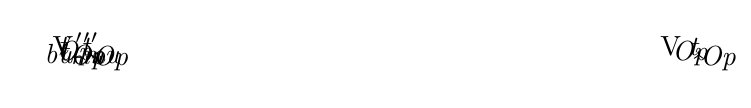
\begin{tikzpicture}
\Tree [.CP \node(op){\emph{Op}}; [.C$'$ \node(bu){\emph{bu-mu}}; [.... ... [.\textit{v}P \node(t){$t_{\textit{Op}}$}; [.\textit{v}P \node(t1){$t_{\text{mu}}$}; [.\textit{v}$'$ \edge[roof]; \node(gap){V $t_{\textit{Op}}$}; ] ] ] ] ] ]
\draw[->,overlay] (gap) to[bend left=40] (t);
\draw[->] (t) to[bend left=40] (op);
\draw[->,dashed] (t1) to[bend left=30] (bu);
\begin{scope}[xshift=3in]
\Tree [.\textit{v}P \node(op){\emph{Op}}; [.\textit{v}P \emph{mu} [.\textit{v}$'$ \edge[roof]; \node(gap){V $t_{\textit{Op}}$}; ] ] ]
\draw[->] (gap) to[bend left=40] (op);
\end{scope}
\end{tikzpicture}
\caption{The CP relatives are plausibly derived by normal \={A}-movement of an operator. I will argue that the same is true for the \textit{v}P-sized counterparts.}
\end{figure}


\section{Diagnosing \={A}-movement} \label{sec:newman:abar}

We hypothesized in the previous section that the gaps in the CP relatives were derived by \={A}-movement. We will now see that the gaps in both the CP relatives and the \textit{v}P-sized clauses have \={A}-properties. Both require resumption when the gap is further embedded, and these resumptive pronouns are sensitive to islands. This additionally motivates a view in which Wolof resumptive pronouns spell out the tails of \={A}-chains in certain contexts. 

Example \REF{ex:newman:femb} shows that adding a layer of embedding requires a resumptive pronoun to be pronounced instead of the gap. Note that this is true for \emph{both} clause types, as seen by the optional presence of the relativizing head \emph{bu}. Also note that the most embedded clause is tensed, indicated by the SP \emph{moo} rather than the infinitival SP \emph{mu}.\footnote{In these examples, the word for `pretend' that our consultant offered was \emph{fog}, which the dictionary claims means `to think, estimate' (\url{http://resourcepage.gambia.dk/ftp/wollof.pdf}). Our consultants never offered \emph{fog} to mean `think', but offered it for sentences like \emph{Roxaya pretended that she caught the fish}. For English sentences containing `think' as an embedding verb, our consultants offered \emph{xalaat}.}

\begin{exe}
	\ex\label{ex:newman:femb} Further embedding: need resumptive pronoun\\
	\gll Jox naa Roxaya j\"en [(b-u) \emph{mu} fog ne moo *(ko) japp] \\
	give \textsc{1sg.pfv} Roxaya fish \textsc{cl-rel} 3\textsc{sg} pretend that 3\textsc{sg.sbj-foc} it catch \\
	\trans `I gave Roxaya a fish to pretend that she caught it.'
\end{exe}

Resumptive pronouns are not unusual in Wolof. Our language consultants offered them frequently in long distance chains of various sorts. Below is an example (p.c. Colin Davis) of a long distance wh-question with a resumptive pronoun in the most embedded clause. 

\begin{exe}
	\ex \label{ex:newman:longwh}
	\gll Lan la suunu yaay wax ne war \emph{na\~nu} \textbf{ko} j\"{e}nd? \\
	what \textsc{C\textsubscript{\normalfont\textit{wh}}.3sg} our mother say that should \textsc{1pl.pfv} it buy \\
	\trans `What did our mother say that we should buy?' 
\end{exe}

Our language consultants also offered long distance gaps, provided we used a different complementizer \emph{la}. There appear to be dialectal differences in whether speakers accept both examples like \REF{ex:newman:longwh} and \REF{ex:newman:longgap} (p.c. Martina Martinovi\'c, Harold Torrence). Our speakers showed a slight preference for examples like \REF{ex:newman:longwh} and so all long-distance dependencies reported henceforth will show resumption. However, future research should investigate the availability of gaps in these contexts as well.

\begin{exe}
	\ex \label{ex:newman:longgap}
	\gll Wu \~nu wax la jig\'e\'en ji b\"egg?\\
	what \textsc{3pl.pfv} say \textsc{C\textsubscript{\normalfont\textit{wh}}.3sg} woman the want\\
	\trans `What did they say that the woman wants?' 
\end{exe}

Resumptive pronouns have frequently been analyzed as triggered by the lack of movement. However, additional investigation of resumptive pronouns in Wolof reveals that they are island sensitive. These findings suggest that resumptive pronouns \emph{can} be derived by movement (following \citealt{sichel:2014} among others).

Example \REF{ex:newman:island} shows us that resumptive pronouns are island sensitive for both the CP and \textit{v}P-sized clauses. Speakers accept example \REF{ex:newman:island} only when the most embedded complementizer is \emph{ne} `that'. Trying to make it \emph{ndax} `if' results in ungrammaticality, despite the fact that there is a resumptive pronoun instead of a gap. This is true both with and without \emph{bu} in the relative clause. Example \REF{ex:newman:rescue} shows that replacing the resumptive pronoun with a full DP makes \emph{ndax} available, showing that only resumptive pronouns are sensitive to islands, not full DPs repeated in situ. 

\begin{exe}
	\ex \label{ex:newman:island} Resumptive pronouns are island sensitive\\
	\gll Jox naa Roxaya j\"en [(b-u) mu fog ne xam-ul \emph{ne/*ndax} ma \textbf{ko} japp] \\
	give \textsc{1sg.pfv} Roxaya fish \textsc{cl-rel} \textsc{3sg} pretend that know-\textsc{neg} that/*if \textsc{1sg} it catch \\
	\trans `I gave Roxaya a fish to pretend that she didn't know that/*if I caught it.'

	\ex \label{ex:newman:rescue} Replacing the resumptive pronoun with a copy of the full DP rescues the sentence\\
	\gll Jox naa Roxaya j\"en bi [mu fog ne xam-ul \emph{ndax} ma japp \textbf{j\"en} \textbf{bi}] \\
	give \textsc{1sg.pfv} Roxaya fish \textsc{def} \textsc{3sg} pretend that know-\textsc{neg} if \textsc{1sg} catch fish \textsc{def} \\
	\trans `I gave Roxaya a fish to pretend that she didn't know if I caught the fish.'
\end{exe}

I therefore propose that gaps in both of these clauses (i.e. with and without \emph{bu}) are derived by \={A}-movement, where long-distance gaps are spelled out as resumptive pronouns. I refer the reader to \citet{sichel:2014} for a specific resumption mechanism. 

If this is true, given that the clauses without \emph{bu} were shown to be bare \textit{v}Ps, \textit{v} must have an independent \={A}-probe that is not dependent on a higher CP probe. This result further supports work that proposes a dedicated A/\={A}-probe on \textit{v} \citep{vanurkrichards:2015,longenbaugh:2917}. However, it is also a departure from the view of Spec \textit{v}P as merely an intermediate landing site for \={A}-movement, and not the final destination. 

A restatement of the proposal is that \={A}-dependencies appear to be tracked at every phase edge regardless of subsequent movement trajectories. This description does not require a novel theory of \={A}-movement, but highlights a hole in our understanding of why such a property exists in grammar. If \={A}-movement to \textit{v} was never observable in the absence of movement to CP, we could imagine that successive cyclic movement through \textit{v}P exists solely due to pressures from linearization. \citet{foxpes:2005} propose that movement to Spec CP cannot proceed if movement does not first target the edge of \textit{v}P, or else the moving element cannot be properly linearized. Though they do not argue that this is the \emph{only} constraint on movement, one could imagine that if it were, movement to Spec \textit{v}P should be optional in the absence of further movement. The \emph{bu}-less clauses in Wolof argue against the possibility that movement to Spec \textit{v}P is generally optional, suggesting that there is still another feature of the grammar governing the distribution of \={A}-probes.

An alternative approach to these facts would be to propose that the \={A}-de\-pen\-den\-cy between the matrix object and the gap in the \emph{bu}-less clauses is not mediated by an operator. Such a theory might posit direct movement of the object from the adjunct clause to a position where it can be selected by a matrix verb (or a determiner in object position on a head-raising analysis of relative clauses (\citealt{kayne:1994,bianchi:1999}, among others). This proposal would avoid the above discussion about motivation for \={A}-movement because there would be an independent reason for the object to move, namely so it is local to higher heads in the matrix clause.

\begin{exe}
	\ex % 
		\tikzstyle{every picture}+=[remember picture, inner sep=0pt, baseline, anchor=base]%
		An alternative derivation for the \emph{bu}-less clauses\\
		{} Kadeer jox na ma  $[_{\textit{vP}}$ \tikz\node(op){j\"en$_i$}; \tikz\node(node2){ma}; $[$ jox Roxaya \tikz\node(node1){$t_i$}; $] ] $\\
		\begin{tikzpicture}[overlay]
\draw[-latex] (node1.south) -- ++(south:1.5ex) -| (op.south);
\end{tikzpicture}
\end{exe}

I will argue against this alternative proposal with evidence from constituency tests. I have been comparing these \emph{bu}-less clauses to relative clauses because of their similar meaning to the clauses with \emph{bu}. Constituency tests, however, reveal that this is likely the wrong characterization. A better analysis might be that they are purpose or rationale clauses that adjoin to a higher position in the matrix clause. Based on these results, it would be unusual for the matrix object to be related to the gap by direct movement, given that the proposed landing position would not c-command the gap, and would also violate an adjunct island (see \figref{fig:newman:10.2}). 

\begin{figure}
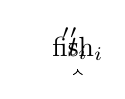
\begin{tikzpicture}
\Tree [.C/TP Kadeer [.C/T$'$ give-\textsc{na}-me [.\textit{v}P [.\textit{v}$'$ \textit{v} [.VP \edge[roof];\node(fish){fish$_i$}; ] ]  [.\textit{v}P to-cook \node(gap){$t_i$}; ] ] ] ]
\draw[->] (gap) to[in=270, out=270] (fish);
\end{tikzpicture}
\caption{Direct movement from the complement of \emph{cook} to the complement of \emph{give} is impossible.} \label{fig:newman:10.2}
\end{figure}

\section{What are the \textit{v}P-infinitives?} \label{sec:newman:vpinfs}

The example in \REF{ex:newman:rel} shows that fronting a nominal modified by one of these adjunct clauses is only possible with \emph{bu}. I conclude therefore, that while the \emph{bu}-clauses are canonical relative clauses that form a constituent with the matrix object, their \emph{bu}-less counterparts are not canonical relative clauses, and must adjoin higher than the matrix object.

\begin{exe}
	\ex \label{ex:newman:rel}
	\gll \textbf{J\"en} [*(b-u) mu togg] mungi ci kaw tabal bi \\
	fish \textsc{cl-rel} \textsc{3sg} cook \textsc{3sg.ipfv} on top table \textsc{def} \\
	\trans `A fish to cook is on the table.'
\end{exe}



Another argument that \emph{bu}-less clauses are not normal relative clauses is that they do not show the same sensitivity to definiteness as regular relative clauses. Wolof relative clauses cannot extrapose across any overt material if the head noun is definite (p.c. Colin Davis), which can be seen in \REF{ex:newman:defrel}. 

	\begin{exe}
		\ex \label{ex:newman:defrel} Relative clause extraposition sensitive to definiteness \begin{xlist}
			\ex[]{
			\gll Gis naa fas d\'emb [w-u nga sopp]\\
			see \textsc{1sg.pfv} horse yesterday \textsc{cl-rel} \textsc{2sg} like\\
			\trans `I saw a horse yesterday that you like.'}
			\ex[]{
			\gll Gis naa fas [w-u nga sopp] \textbf{wi} d\'emb\\
			see \textsc{1sg.pfv} horse \textsc{cl-rel} \textsc{2sg} like \textsc{def} yesterday\\
			\trans `I saw the horse that you like yesterday.'}
			\ex[*]{
			\gll Gis naa fas \textbf{wi} d\'emb [w-u nga sopp]\\
			see \textsc{1sg.pfv} horse \textsc{def} yesterday \textsc{cl-rel} \textsc{2sg} like\\
			\trans intended: `I saw the horse yesterday that you like.'}
		\end{xlist}
\end{exe}
	
By contrast, the \emph{bu}-less clauses may be separated from a definite head noun by other arguments, surfacing all the way to the right of the clause, as in \REF{ex:newman:extra}. Here, the speaker offered an optional complementizer \emph{pur} (borrowed from French) but rejected \emph{bu}.
	
\begin{exe}
	\ex \label{ex:newman:extra}
	\gll Tekk naa $[$j\"en bi$]$ ci tabal bi $[$(pur/*bu) mu togg$]$ \\
	put \textsc{1sg.pfv} fish \textsc{def} on table \textsc{def} (for/*\textsc{rel}) \textsc{3sg} cook \\
	\trans `I put the fish on the table to cook.'
\end{exe}

I therefore conclude that the \emph{bu}-less clauses are not relative clauses. They do not form a constituent with the head noun and can show up further to the right than normal relative clauses do. It seems they must therefore be merged higher than the object, possibly adjoining to the matrix \textit{v}P as an adjunct. 

Adjunct infinitives are very common in English and can have a range of meanings \citep{huettner:1989}, including purpose or rationale interpretations. It seems that the \emph{bu}-less clauses might therefore be analogously described as having a covert \emph{in order to/for the purpose of}, as paraphrased in \REF{ex:newman:par}.\footnote{It is possible that the English translation of (\ref{ex:newman:bu}a) is itself structurally ambiguous in the way that Wolof makes explicit. If so, the proposal for the \emph{bu}-less clauses in Wolof will presumably work for its English counterpart as well, though the tests may be harder to apply in English.}

\begin{exe}
	\ex \label{ex:newman:par} Paraphrase of (\ref{ex:newman:bu}b)\\
	\gll Kadeer jox na ma j\"en [ma jox Roxaya] \\
	K give \textsc{3sg.pfv} me fish \textsc{1sg} give R \\
	\trans `Kadeer gave me a fish in order for me to give it to Roxaya.'
\end{exe}

The fact that Wolof has adjunct infinitives is unsurprising, but the fact that these adjunct infinitives show an \={A}-dependency with a nominal in the matrix clause merits further discussion. Particularly unusual about this configuration is the fact that the gap in the adjunct clause is presumably not c-commanded by the matrix object. A potential way of modeling this behavior is shown in \figref{fig:newman:10.3}, where the gap is treated as parasitic, licensed by covert movement of the matrix object. 


\begin{figure} 
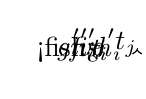
\begin{tikzpicture}
\Tree [.\textit{v}P \node(vp){<fish>\textsubscript{$i$}}; [ [.\textit{v}P [.\textit{v}$'$ \node(v){\textit{give}}; [.ApplP \textit{Kadeer} [.Appl$'$ Appl [.V$'$ \node(V){$t$}; \node(d){\textit{fish}\textsubscript{$i$}}; ] ] ] ] ] [.\textit{v}P \textit{Op}\textsubscript{$j$} [.\textit{v}P \textit{mu} [.\textit{v}$'$ \textit{cook} [.VP \edge[roof]; {...$t_j$} ] ] ] ] ] ]
\draw [->] (d) to[bend left=65] (vp);
\draw [->] (V) to[bend left=45] (v); 
\end{tikzpicture}
\caption{A schematic of \citegen{nissenbaum:2000} parasitic gap configuration with the \textsc{mu}-clause as the parasitic gap-containing \textit{v}P adjunct.} \label{fig:newman:10.3}
\end{figure}

Treating these \emph{bu}-less clauses as adjuncts with parasitic gaps may explain why the adjunct clause is obligatorily small. Recall that these clauses rejected aspect, which was one piece of evidence that they are \textit{v}P-sized. This may be the case because the clause has to attach at matrix \textit{v}P in order for the gap to be licensed. Predicate modification should therefore require the two clauses to be of the same type.

Future research is needed to verify this analysis, given that there is no independent evidence currently available to suggest that the object moves in the matrix clause, which is theoretically necessary to license the parasitic gap. If such evidence were found, it would be further evidence in support of the proposal that covert movement can license parasitic gaps, which is independently motivated in \citet{nissenbaumschwarz:2010} for English gapped degree phrases. 

This analysis would suggest that infinitival clauses with parasitic gaps should be more common than has been reported. In languages such as English, which do not morphologically distinguish different kinds of infinitives, it is difficult to tell whether they exist, given their surface similarity to infinitival relatives. 

German, however, has two morphologically distinct infinitival clauses in the way that Wolof does. Like in Wolof, only the morphologically more complex one can form a constituent with a nominal (p.c. Johannes Hein). 

\begin{exe}
	\ex
	\gll Ich hab dir einen Fisch [zu/zum kochen gegeben]\\
	I have you.\textsc{dat} a.\textsc{acc} fish to/to.\textsc{dat} cook given\\
	\trans `I gave you a fish to cook.'
	\ex
	\gll [Ein Fisch zum/*zu kochen] liegt auf dem Tisch \\
	a fish to.\textsc{dat}/*to cook lies on the table\\
	\trans `A fish to cook is on the table.'
\end{exe}

The \emph{zu}-infinitives in these examples appear prima facie to be good candidates for parasitic gap constructions. Investigating the structural properties of these clauses in relation to the properties of the gaps inside them should be a fruitful area for future research.

\section{Conclusion} \label{sec:newman:conc}

In this paper, I have investigated two Wolof adjunct clauses. These two clauses are very similar on the surface, differing only in the presence or absence of a relativizing complementizer (\emph{bu}), and can be uttered in similar situations. While many languages have constructions with optional complementizers, I argued against a unified account of these constructions by showing that the presence or absence of the complementizer has syntactic consequences, which would be unexpected if it was truly optional. 

Based on evidence from clitic climbing, the availability of aspectual markers, and constituency tests, I have argued that one of these constructions (the one with \emph{bu}) should be treated as a relative clause, while the other should be treated as an infinitival adjunct, like a purpose clause. Following Martinovi\'c, I additionally argued that the latter clause type was \textit{v}P-sized, unlike relative clauses, which I assume to be full CPs. 

Despite their difference in size, I further showed that the gaps inside both constructions show signatures of \={A}-movement. Both require resumption when further embedded, but the resumptive pronouns are island sensitive, suggesting that they still participate in an \={A}-chain. Given that one of these clauses was argued to be \textit{v}P sized, this finding requires a novel theoretical assumption, which is that \={A}-movement can not only move through Spec \textit{v}P but can stop there as well.\pagebreak


\section*{Abbreviations}

\begin{multicols}{2}
\begin{tabbing}
\textsc{ndef}\hspace{1ex}\=Indefinite determiner\kill
\textsc{acc}  \> Accusative \\
\textsc{ben}  \> Benefactive \\
\textsc{C} \> Complementizer\\
\textsc{cl} \> Noun class \\
\textsc{dat}  \> Dative \\
\textsc{def}  \> Definite determiner \\
\textsc{foc}  \> Focus \\
\textsc{fut}  \> Future\\
\textsc{ndef}  \> Indefinite determiner \\
\textsc{neg} \> Negation\\
\textsc{pfv}  \> Perfective \\
\textsc{pl} \> Plural\\
\textsc{rel}  \> Relativizer \\
\textsc{sbj} \> Subject \\
\textsc{sg} \> Singular\\
\textsc{v} \> Verb
\end{tabbing}
\end{multicols}

\section*{Acknowledgments}

My thanks go to Yadav Gowda, Johannes Hein, Martina Martinovi\'c, David Pesetsky, Norvin Richards, Harrold Torrence, and the audience at ACAL 2019 for helpful insight and discussion. A very special thank you to our Wolof consultants for sharing their language and enthusiasm: Lamine Diallo, Aicha Seck, and Lamine Tour\'e! All mistakes are my own.



\section*{Appendix: A different \emph{bu}-less \textsc{mu} clause}

Plugging the gap allows the \emph{bu}-less clauses to host aspect.

\begin{exe}
	\ex 
	\gll Roxaya jox na Kadeer j\"en mu \textbf{ko}-y togg \\
	R give \textsc{3sg.pfv} K fish \textsc{3sg} it\textsc{-ipfv} cook \\
	\trans `$\approx$ Roxaya gave Kadeer a fish, he cooks it.'
\end{exe}

Note the different translation, however. This construction seems to be different than those discussed so far in this paper. Additionally, the object clitic seems not to be a resumptive pronoun based on several properties.

\begin{itemize}
	\item Cannot appear in clauses with \emph{bu} (unlike other resumptive pronouns we saw)
	\item Ruled out if the matrix clause is negative
	\item Allowed for a different set of matrix predicates than gaps
\end{itemize}

\begin{exe}
	\ex \begin{xlist}
		\ex[*]{
		\gll Roxaya jox na Kadeer j\"en \textbf{b-u} mu togg ko \\ 
		R give \textsc{3sg.pfv} K fish \textsc{cl-rel} \textsc{3sg} cook it \\
		\trans `Intended: Roxaya gave K a fish to cook.'}
		\ex[]{
		\gll Jox-uma Roxaya j\"en mu togg (*ko) \\
		give-\textsc{neg.1sg.pfv} Roxaya fish \textsc{3sg} cook (*it) \\
		\trans `I didn't give Roxaya a fish to cook.'}
	\end{xlist}
	\ex \label{res} \begin{xlist}
		\ex[]{ 
		\gll togg naa j\"en, ma lekk (ko) \\
		cook \textsc{1sg.pfv} fish, \textsc{1sg} eat (it) \\
		\trans `I cooked a fish \{to eat/I eat it\}.'}
		\ex[]{
		\gll sopp naa j\"en, ma lekk *(ko) \\
		like \textsc{1sg.pfv} fish, \textsc{1sg} eat *(it) \\
		\trans `I like fish \{ * to eat/\langscicheckmark I eat it\}.'}
	\end{xlist}	
\end{exe}

This seems to be some sort of subordinate clause where the object pronoun is coreferent with the matrix object, but not derived by movement. The fact that the pronoun is sensitive to matrix negation makes sense if it is referential. In other words, if Kadeer did not give someone a fish, there is no salient fish that a pronoun can refer to.

Similarly, these pronouns show different sensitivity to the matrix predicate than gaps do. While predicates like \emph{cook} can take an infinitival adjunct that optionally has a pronoun or a gap, \emph{like} requires a pronoun in the adjunct clause.



{\sloppy\printbibliography[heading=subbibliography,notkeyword=this]}

\end{document}
